\section{Auswertung}
\label{sec:Auswertung}
Im Versuch wurde für die Datenaufzeichnung ein XY-Schreiber verwendet. Um diese Werte zu
digitalisieren wurde das Tool WebPlotDigitizer \cite{Rohatgi2020} verwendet.

\subsection{Mittlere freie Weglänge}
\label{sec:Mittlere freie Weglänge}
Als allererstes soll die mittlere freie Weglänge der Elektronen in der Apperatur berechnet
werden. Mit der Formel
\[
	w / \si{\centi\meter} = \frac{0,0029}{p_\text{sät}} = \frac{0,0029}{5,5 \cdot 10^7
	\cdot \exp(-6876 / T)}
\]
folgen die Werte in \autoref{tab:mfp}. Zum Vergleich wird die Anzahl an Stößen auf einer
Distanz von $\SI{1}{\centi\meter}$ angegeben.
\begin{table}
	\centering
	\caption{Mittlere freie Weglänge der Elektronen bei den hier relevanten
	Temperaturen.}
	\label{tab:mfp}
	\sisetup{table-format=2.1}
	\begin{tabular}{c c c}
		\toprule
		$T / \si{^\circ C}$ & $\overline{w} / \si{\centi\meter}$ & $n \cdot
		\si{\centi\meter}$ \\
		\midrule
		25    & 0,55 & 1,81 \\
		148   & $6,53 \cdot 10^{-4}$ & $1,53 \cdot 10^{3}$ \\
		168   & $3,12 \cdot 10^{-4}$ & $3,21 \cdot 10^{3}$ \\
		197,5 & $1,17 \cdot 10^{-4}$ & $8,53 \cdot 10^{3}$ \\
		\bottomrule
	\end{tabular}
\end{table}

\subsection{Integrale Energieverteilung}
\label{sec:Integrale Energieverteilung}
In diesem Versuchsteil wurde bei $U_B = \SI{9}{\volt} \text{ bzw. } \SI{12}{\volt}$ und $T
= 25^\circ \symup{C} \text{ bzw. } 148^\circ \symup{C}$ die Abbremsspannung $U_A$
variiert. Wie oben erklärt wurden die Werte mit WebPlotDigitizer extrahiert. Diese sind in
\autoref{tab:25} und \autoref{tab:148} angegeben. Als Ableitung wurde der einseitige
Differenzenquotient
\[
	y^\prime_i = \frac{y_{i+1} - y_i}{x_{i+1} - x_i}
\]
für jeden Wert berechnet. Da hier nur der qualitative relevant ist, wurden die Werte $y$
und $y^\prime$ mit der $L_\infty$-Norm für bessere Lesbarkeit normiert. Sie wurden in
\autoref{fig:0025} und \autoref{fig:1480} grafisch dargestellt. 
\\
Im Plot für die Messung bei Zimmertemperatur ist der rapide Abfall bei $U_A =
\SI{6,739}{\volt}$ auffällig, was darauf hindeutet, dass die Elektronen vorwiegend die
Energie $\SI{6,739}{eV}$ besitzen. Die Beschleunigungspannung lag jedoch bei
$\SI{9}{\volt}$, aus der Differenz folgt das Kontaktpotential
\begin{equation}
	K = (9 - 6,739) \, \symup{V} = \SI{2.261}{\volt}.
\end{equation}
Dass der Abfall jedoch nicht instantan stattfindet liegt an der Energieverteilung der
Elektronen und dadran, dass nur die Geschwindigkeit in Richtung des Rohres hier beiträgt,
die tatsächliche Bewegung aber zufallsverteilt ist.
\begin{figure}[H]
	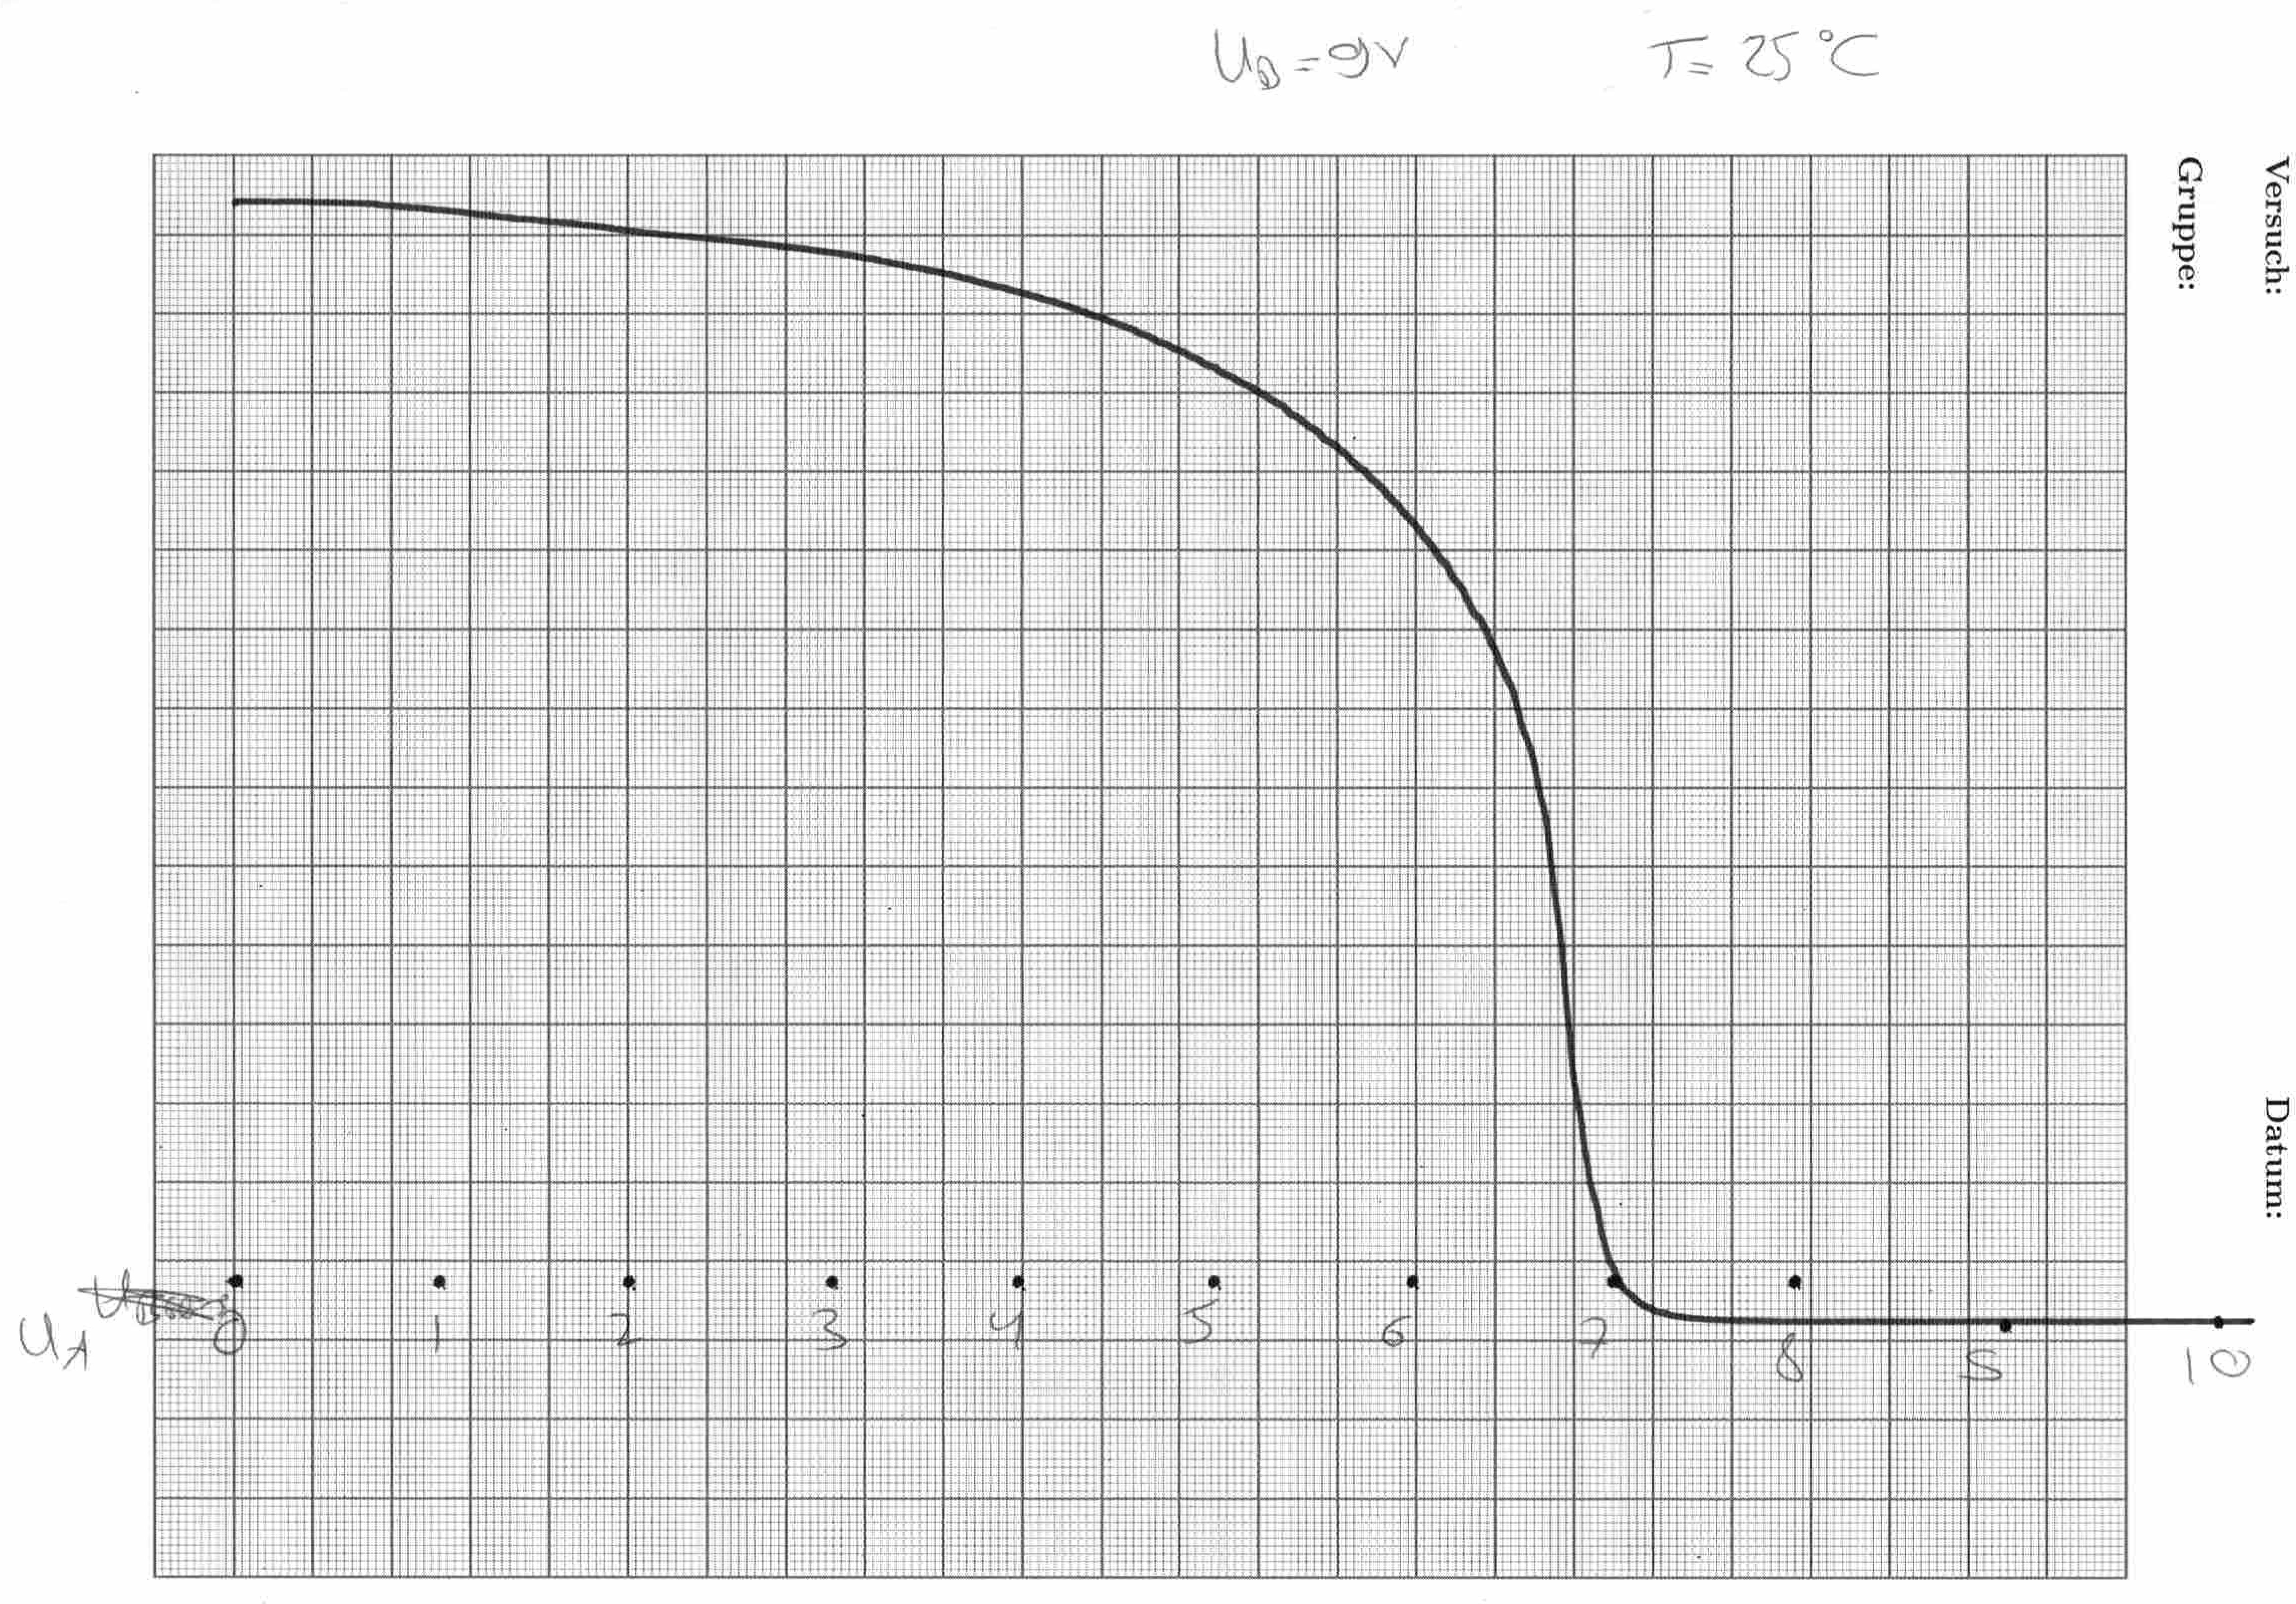
\includegraphics{build/0025.pdf}
	\caption{Der Elektronenstrom und seine Ableitung in Abhängigkeit von der
	Bremsspannung $U_A$, bei der Temperatur $T=25^\circ \symup{C}$.}
	\label{fig:0025}
\end{figure}
\begin{figure}[H]
	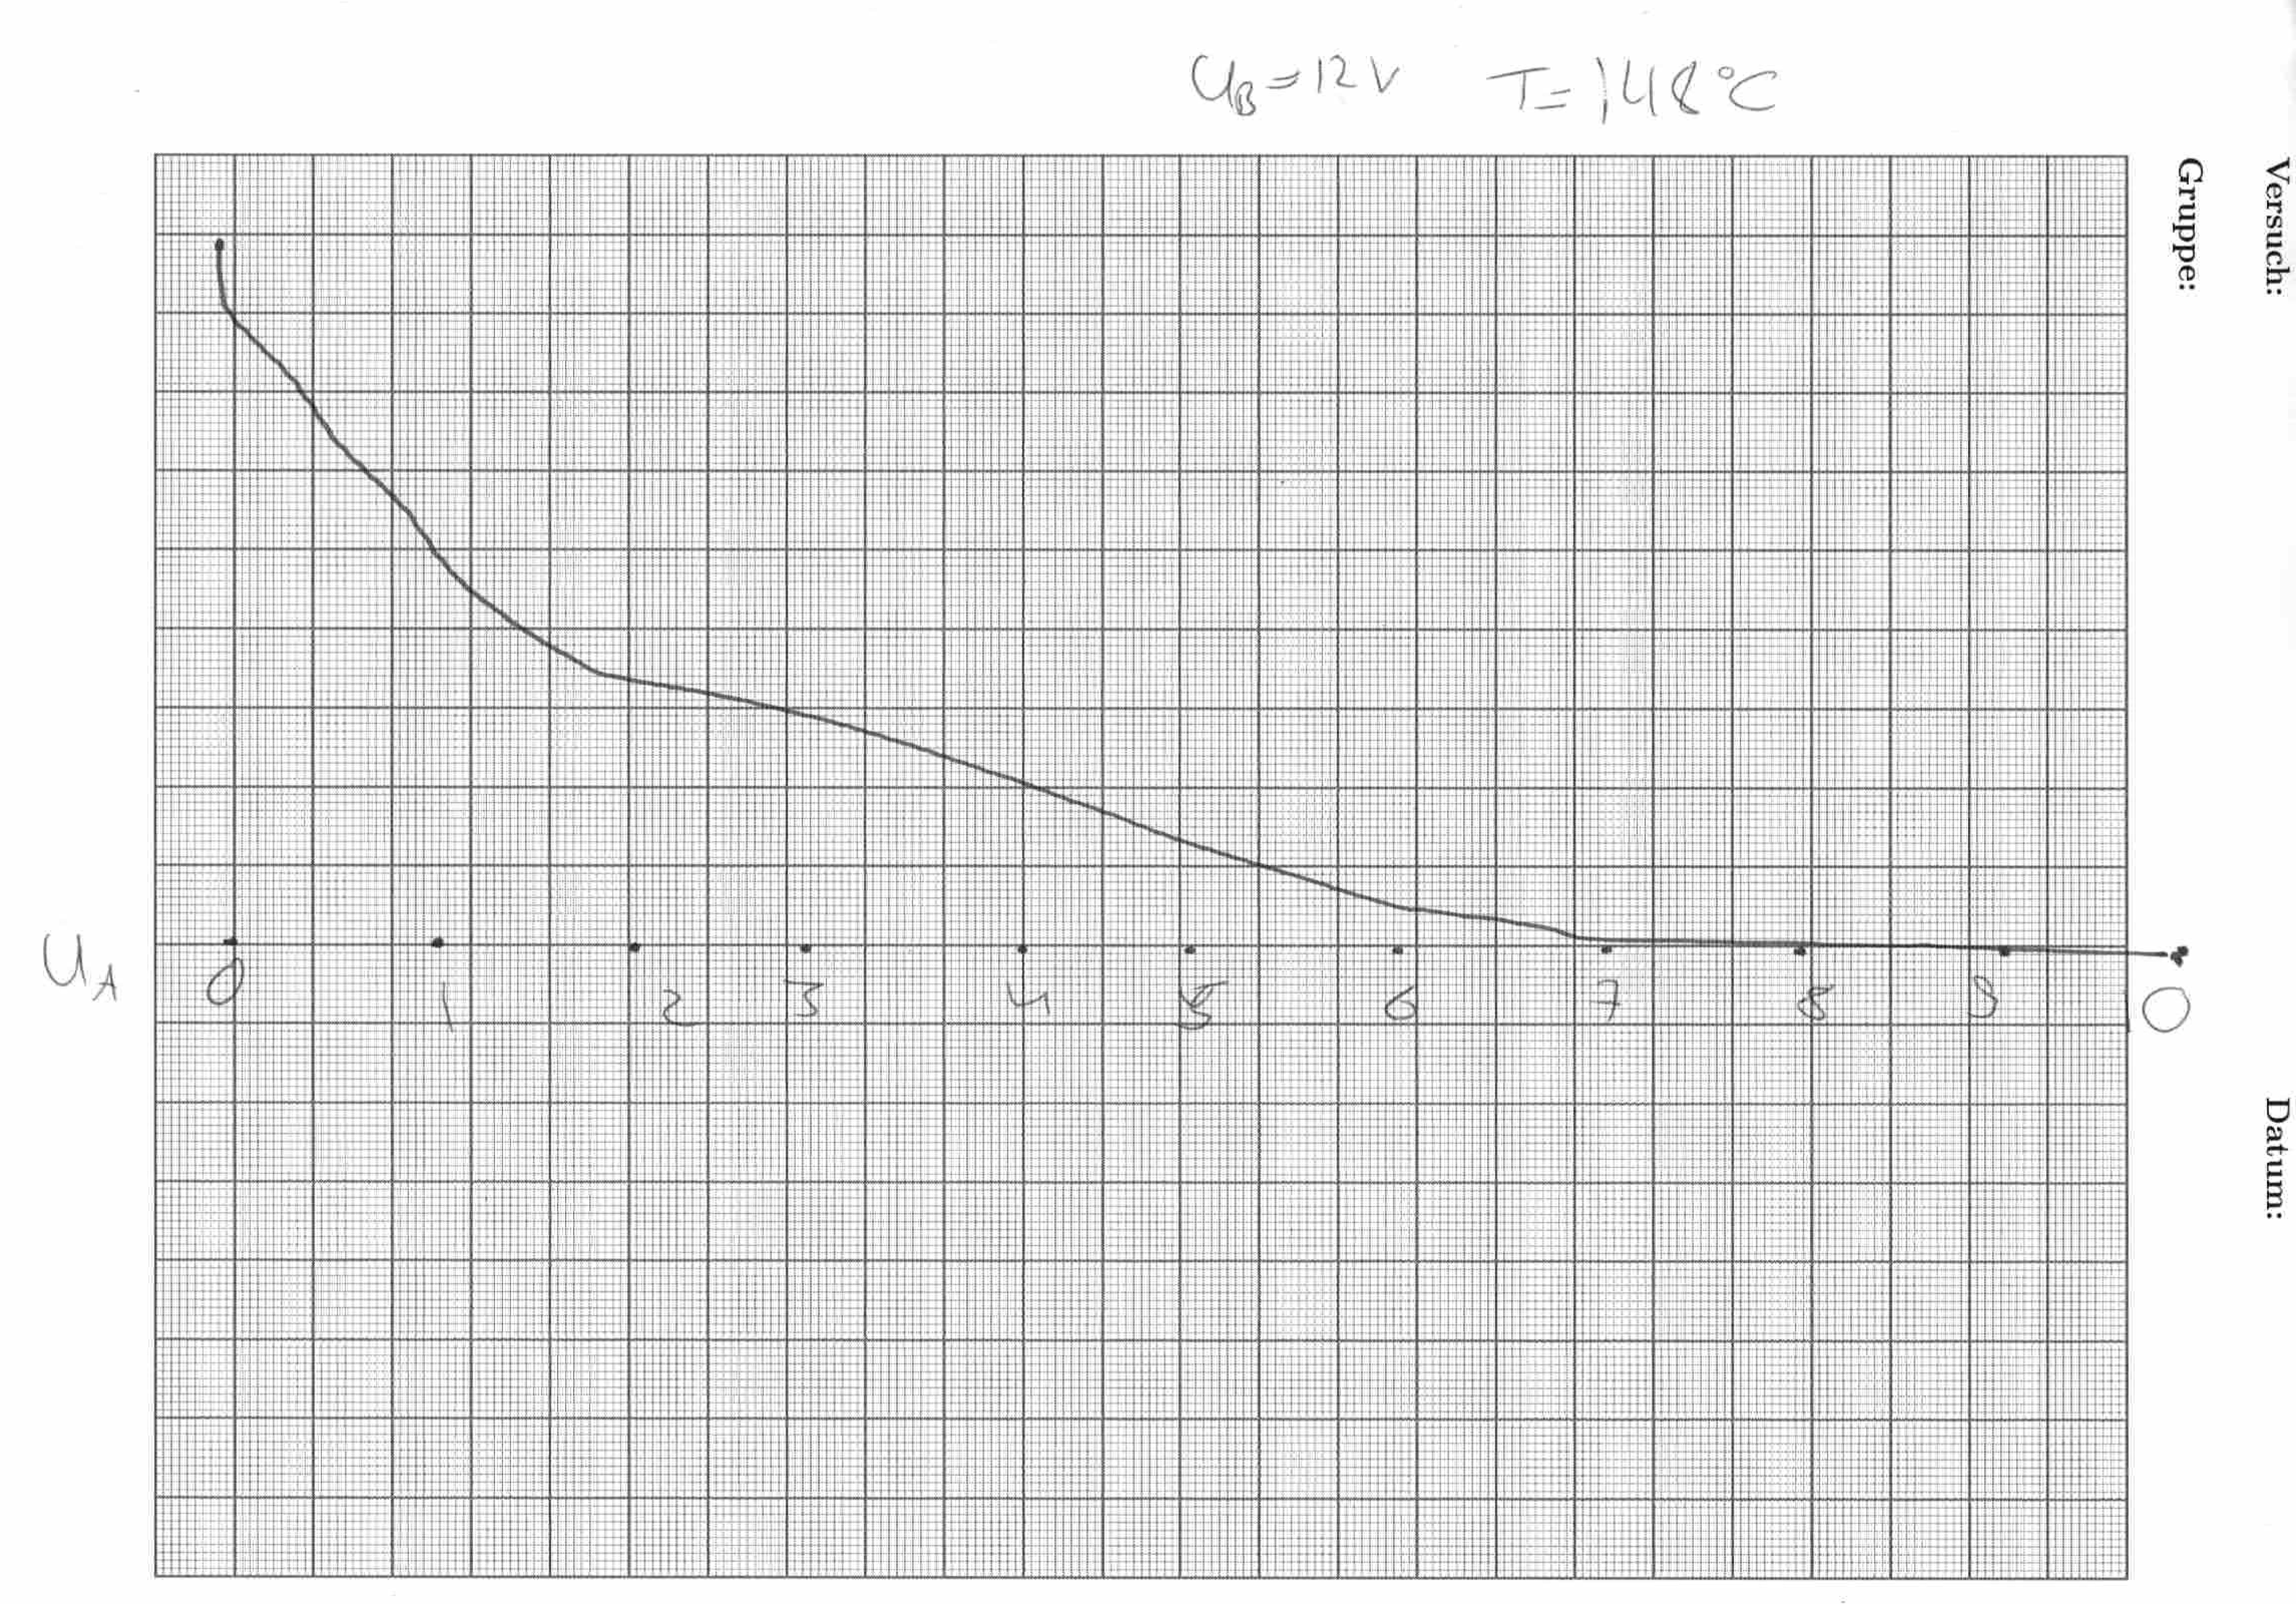
\includegraphics{build/1480.pdf}
	\caption{Der Elektronenstrom und seine Ableitung in Abhängigkeit von der
	Bremsspannung $U_A$, bei der Temperatur $T=148^\circ \symup{C}$ .}
	\label{fig:1480}
\end{figure}

\begin{longtable}{c c c}
	\caption{Messdaten für $25^\circ \symup{C}$.}
	\label{tab:25}\\
	\hline
	$x$ & $y$  & $\Delta y / \Delta x$ \\
	\hline
	% data
	-0,058&1,000&0,000 \\
	0,341&1,000&-0,005 \\
	0,750&0,996&-0,010 \\
	1,170&0,989&-0,011 \\
	1,559&0,982&-0,014 \\
	1,938&0,973&-0,007 \\
	2,367&0,967&-0,014 \\
	2,781&0,957&-0,014 \\
	3,185&0,948&-0,020 \\
	3,586&0,934&-0,026 \\
	3,790&0,925&-0,026 \\
	3,996&0,916&-0,030 \\
	4,194&0,906&-0,036 \\
	4,405&0,893&-0,040 \\
	4,597&0,880&-0,050 \\
	4,798&0,863&-0,017 \\
	0,141&1,000&-0,002 \\
	0,548&0,998&-0,006 \\
	0,957&0,994&-0,013 \\
	1,350&0,986&-0,011 \\
	1,751&0,978&-0,014 \\
	2,183&0,968&-0,009 \\
	2,592&0,962&-0,012 \\
	2,976&0,954&-0,019 \\
	3,397&0,941&-0,035 \\
	4,990&0,846&-0,061 \\
	5,210&0,823&-0,064 \\
	5,397&0,802&-0,079 \\
	5,609&0,774&-0,095 \\
	5,815&0,740&-0,113 \\
	6,015&0,701&-0,148 \\
	6,227&0,648&-0,177 \\
	6,436&0,585&-0,187 \\
	6,324&0,620&-0,161 \\
	6,124&0,675&-0,392 \\
	6,820&0,209&-0,688 \\
	6,536&0,543&-0,414 \\
	6,617&0,486&-0,531 \\
	6,684&0,425&-0,768 \\
	6,739&0,352&-1,000 \\
	6,778&0,286&-0,811 \\
	6,881&0,143&-0,826 \\
	6,918&0,092&-0,373 \\
	6,979&0,053&-0,526 \\
	7,009&0,025&-0,330 \\
	7,051&0,002&-0,076 \\
	7,302&-0,031&-0,009 \\
	7,643&-0,036&0,001 \\
	7,892&-0,036&-0,004 \\
	8,048&-0,037&0,004 \\
	8,257&-0,036&0,000 \\
	8,449&-0,036&-0,001 \\
	8,867&-0,037&-0,005 \\
	9,059&-0,038&0,003 \\
	9,271&-0,037&0,000 \\
	9,681&-0,037&-0,001 \\
	10,146&-0,038& \\
\end{longtable}

\begin{longtable}{c c c}
	\caption{Messdaten für $148^\circ \symup{C}$.}
	\label{tab:148}\\
	\hline
	$x$ & $y$  & $\Delta y / \Delta x$ \\
	\hline
	% data
	-0,009&1,000&-1,000 \\
	0,066&0,889&-0,190 \\
	0,261&0,835&-0,232 \\
	0,462&0,766&-0,244 \\
	0,656&0,697&-0,197 \\
	0,851&0,641&-0,244 \\
	1,032&0,576&-0,227 \\
	1,246&0,504&-0,152 \\
	1,445&0,460&-0,119 \\
	1,644&0,425&-0,080 \\
	2,045&0,378&-0,036 \\
	2,233&0,368&-0,029 \\
	2,445&0,359&-0,038 \\
	2,656&0,347&-0,039 \\
	2,844&0,337&-0,050 \\
	3,042&0,322&-0,056 \\
	3,242&0,305&-0,053 \\
	3,443&0,290&-0,064 \\
	3,647&0,271&-0,067 \\
	3,825&0,253&-0,063 \\
	4,042&0,233&-0,067 \\
	4,230&0,215&-0,071 \\
	4,440&0,193&-0,072 \\
	4,631&0,173&-0,072 \\
	4,832&0,151&-0,058 \\
	5,013&0,136&-0,058 \\
	5,240&0,117&-0,056 \\
	5,441&0,100&-0,063 \\
	5,638&0,082&-0,040 \\
	5,853&0,069&-0,047 \\
	6,037&0,056&-0,033 \\
	6,226&0,047&-0,026 \\
	6,437&0,039&-0,024 \\
	6,639&0,032&-0,055 \\
	6,843&0,016&-0,014 \\
	7,048&0,011&-0,001 \\
	7,349&0,011&-0,005 \\
	7,449&0,010&-0,009 \\
	7,647&0,008&0,008 \\
	7,823&0,010&-0,002 \\
	8,041&0,009&-0,002 \\
	8,243&0,008&-0,005 \\
	8,452&0,007&-0,002 \\
	8,657&0,006&-0,009 \\
	8,853&0,004&-0,002 \\
	9,074&0,003&-0,010 \\
	9,250&0,000&-0,008 \\
	9,465&-0,002&-0,002 \\
	9,657&-0,003&-0,002 \\
	9,872&-0,003& \\
\end{longtable}
